\documentclass[a4paper,10pt]{article}

\usepackage[activeacute]{babel}
\usepackage[utf8]{inputenc}
\usepackage{bookman}
\usepackage{color}
\usepackage{graphicx,wrapfig}
\usepackage{anysize}
\usepackage[pdftex=true,colorlinks=true,linkcolor=black,urlcolor=blue,bookmarksopen=true]{hyperref}
\usepackage{bookmark}
\usepackage{amssymb,amsmath,mathtools,cancel}
\usepackage[dvipsnames]{xcolor}

\setlength\parindent{0pt}

\begin{document}

\section*{\underline{Planteamiento A:}}

\begin{wrapfigure}{r}{5.5cm}
    \vspace{-15pt}
    \centering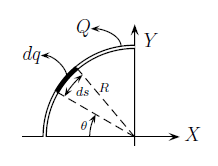
\includegraphics[width=\linewidth]{Graphics/PlanteamientoA.png}
    \vspace{-40pt}
\end{wrapfigure}

En la figura adjunta se muestra un alambre en forma
de un arco de circunferencia, cuyo radio es $R$. El alambre tiene una carga $Q$
distribuida en todo el alambre, pero no necesariamente uniforme. Considere
que la posición angular $\theta$, definida como positiva, es medida respecto al
semieje horizontal negativo según lo indicado en la figura. Sobre la base de
este planteamiento responda las siguientes preguntas:

\begin{itemize}
    \item[(1a)]La densidad lineal media del alambre viene dada por:
\end{itemize}

La densidad lineal media es $\langle\lambda\rangle=\frac{Q}{s}$.
Para calcular la longitud del arco de circunferencia $L_{s}$, nos fijamos en el hecho
que dicho arco corresponde a un cuarto de la longitud de la circunferencia completa.
De esta forma:

\begin{equation*}
    L_{s}=\frac{L_c}{4}=\frac{2\pi R}{4}=\frac{\pi R}{2}
\end{equation*}

Luego,

\begin{equation*}
    \langle\lambda\rangle=\frac{Q}{L_{s}}=\frac{Q}{\frac{\pi R}{2}}=\frac{2Q}{\pi R}
    \quad\therefore\quad\boxed{\langle\lambda\rangle=\frac{2Q}{\pi R}}
\end{equation*}

\begin{itemize}
    \item[(1b)]Si la carga se distribuye de manera uniforme sobre el alambre,
    la carga contenida en el alambre hasta un ángulo $\theta$ viene dada por:
\end{itemize}

Basta recordar que un segmento $s$ de arco puede escribirse en t\'erminos del
radio $R$ y del \'angulo $\theta$ necesario para construirlo, esto es $s=R\theta$. Adem\'as,
cuando se trata de un elemento infinitesimal $\mathrm{d}s$, entonces su valor corresponde a
$ds=R\mathrm{d}\theta$. Ahora, calculamos la densidad de carga lineal local:

\begin{equation*}
    \lambda=\frac{\mathrm{d}q}{\mathrm{d}s}=\frac{\mathrm{d}q}{R\mathrm{d}\theta}
\end{equation*}

Tambi\'en hay que recordar que, cuando la carga se distribuye uniformemente sobre
el espacio que la contiene, el valor de la distribuci\'on de carga local coincide
con el de la carga media. As\'i, pues:

\begin{equation*}
    \lambda=\langle\lambda\rangle\Longrightarrow
    \frac{\mathrm{d}q}{\cancel{R}\mathrm{d}\theta}=\frac{2Q}{\pi \cancel{R}}
    \quad\therefore\quad\mathrm{d}q=\frac{2Q}{\pi}\mathrm{d}\theta
\end{equation*}

Finalmente, integramos ambos miembros de la ecuaci\'on definiendo adecuadamente
los l\'imites de integraci\'on:

\begin{equation*}
    \int_{0}^{Q_{\theta}} \mathrm{d}q = \int_{0}^{\theta} \frac{2Q}{\pi}\mathrm{d}\theta
    \Longrightarrow \boxed{Q_{\theta}=\frac{2Q}{\pi}\theta}
\end{equation*}

\textbf{Observaci\'on:} Los valores de carga $Q$ y $Q_{\theta}$ son los mismos,
pero para efectos de la soluci\'on del ejercicio se denotan diferente.

\begin{itemize}
    \item[(1c)]Si la carga se distribuye de forma tal que la densidad lineal local
    varía proporcionalmente según el $\sin\theta$, entonces, dicha densidad como función
    del ángulo $\theta$ viene por:
\end{itemize}

Tenemos que $\lambda(s)\varpropto\sin\theta\therefore\lambda(s)=\lambda_{0}\sin\theta$.
Por regla de la cadena, podemos poner a la cantidad $\lambda(s)$ en funci\'on de
$\theta$, de esta forma:

\begin{equation*}
    \lambda(s)=\frac{\mathrm{d}Q}{\mathrm{d}s}
    =\frac{\mathrm{d}Q}{\mathrm{d}\theta}\frac{\mathrm{d}\theta}{\mathrm{d}s}
    =\frac{\mathrm{d}Q}{\mathrm{d}\theta}\frac{1}{R}
    \Longrightarrow\mathrm{d}Q=R\lambda(s)\mathrm{d}\theta
\end{equation*}

En donde usamos el hecho que
$\mathrm{d}s=R\mathrm{d}\theta\Longrightarrow\frac{\mathrm{d}\theta}{\mathrm{d}s}=\frac{1}{R}$.
Ahora, imponemos que la carga se distribuye por todo el \'angulo $\theta=\frac{\pi}{2}$
e integramos definiendo adecuadamente los l\'imites de integraci\'on:

\begin{equation*}
    \int_{0}^{Q}\mathrm{d}Q=\int_{0}^{\theta=\frac{\pi}{2}}R\lambda(s)\mathrm{d}\theta
    \Longrightarrow Q=R\int_{0}^{\frac{\pi}{2}}\lambda_{0}\sin\theta\mathrm{d}\theta
    =R\lambda_{0}\int_{0}^{\frac{\pi}{2}}\sin\theta\mathrm{d}\theta
    =-R\lambda_{0}\left[\cos\frac{\pi}{2}-\cos0\right]
\end{equation*}

\begin{equation*}
    =-R\lambda_{0}[-1]
    =R\lambda_{0}
    \Longrightarrow Q=R\lambda_{0}
    \quad\therefore\quad\lambda_{0}=\frac{Q}{R}
\end{equation*}

Por \'ultimo,

\begin{equation*}
    \boxed{\lambda(s(\theta))=\frac{Q}{R}\sin\theta}
\end{equation*}

\begin{itemize}
    \item[(1d)]Si la carga se distribuye de forma tal que ésta varia proporcionalmente
    según el $\sin\theta$, la densidad local de carga como función del ángulo $\theta$ viene por:
\end{itemize}


Como ahora es la carga la que es proporcional al $\sin\theta$, entonces se cumple
que $Q(\theta)\varpropto\sin\theta\therefore Q(\theta)=Q_{0}\sin\theta$,
donde $Q_{0}$ es otra constante a determinar y lo podemos hacer nuevamente
imponiendo la misma condici\'on $\theta=\frac{\pi}{2}$ para el valor de $Q$:

\begin{equation*}
    Q(\theta=\frac{\pi}{2})=Q\Longrightarrow Q_{0}\sin\frac{\pi}{2}=Q
    \Longrightarrow Q_{0}=Q \Longrightarrow Q(\theta)=Q\sin\theta
\end{equation*}

Tambi\'en cabe recordar que
$\mathrm{d}s=R\mathrm{d}\theta\Longrightarrow\frac{\mathrm{d}\theta}{\mathrm{d}s}=\frac{1}{R}$.
Finalmente, por regla de la cadena, la densidad de carga lineal local, escrita en
funci\'on del segmento de arco $s$, podemos escribirla a su vez en funci\'on de $\theta$:

\begin{equation*}
    \lambda(s)=\frac{\mathrm{d}Q}{\mathrm{d}s}
    \Longrightarrow\lambda(s(\theta))
    =\frac{\mathrm{d}Q(\theta)}{\mathrm{d}\theta}\frac{\mathrm{d}\theta}{\mathrm{d}s}
    =Q\cos\theta\frac{1}{R}\quad\therefore\quad
    \boxed{\lambda(s(\theta))=\frac{Q}{R}\cos\theta}
\end{equation*}

\section*{\underline{Planteamiento B:}}

\begin{wrapfigure}{r}{5.5cm}
    \centering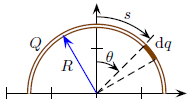
\includegraphics[width=\linewidth]{Graphics/PlanteamientoB.png}
    \vspace{-15pt}
\end{wrapfigure}

En la figura adjunta se muestra un semi-aro de radio $R$
y con una carga positiva $Q$ distribuida en toda su longitud. Considere que
un elemento infinitesimal de carga $\mathrm{d}q$ se encuentra localizado en una ángulo
$\theta$, dicho ángulo es medido respecto a la vertical tal como se indica en la
figura adjunta. También considere que la longitud de arco $s$ sobre el alambre
es medido respecto al eje vertical, tal como se indica. Sobre la base de este
planteamiento responda las siguientes preguntas:

\begin{itemize}
    \item[(2a)] Si la carga $Q$ se distribuye uniformemente sobre el semi-aro, el valor
    para la carga contenida hasta la abertura $\theta$ viene dada por: 
\end{itemize}

Como la carga se distribuye uniformemente, se cumple que $\lambda=\langle\lambda\rangle$.
Esto es:

\begin{equation*}
    \begin{cases}
        \langle\lambda\rangle=\dfrac{Q}{L_{arc}}=\dfrac{Q}{\frac{\cancel{2}\pi R}{\cancel{2}}}
        =\dfrac{Q}{\pi R}\\
        \lambda=\dfrac{\mathrm{d}q}{\mathrm{d}s}=\dfrac{\mathrm{d}q}{R\mathrm{d}\theta}
    \end{cases}
    \Longrightarrow \lambda=\langle\lambda\rangle \Longrightarrow
    \dfrac{Q}{\pi \cancel{R}}=\dfrac{\mathrm{d}q}{\cancel{R}\mathrm{d}\theta}
    \Longrightarrow \mathrm{d}q=\frac{Q}{\pi}\mathrm{d}\theta
\end{equation*}

Luego, integramos definiendo los l\'imites adecuadamente:

\begin{equation*}
    \int_{0}^{Q_{\theta}} \mathrm{d}q = \int_{0}^{\theta} \frac{Q}{\pi}\mathrm{d}\theta
    \Longrightarrow\boxed{Q_{\theta}=\frac{Q}{\pi}\theta}
\end{equation*}

\begin{itemize}
    \item[(2b)] Si la carga $Q$ se distribuye a lo largo de alambre con una densidad
    lineal de carga local dada por $\lambda(s)=\lambda_{0}\cos\left(\frac{s}{R}\right)$, donde
    $s$ es la longitud de arco sobre el alambre indicado en la figura. El valor
    de la constante $\lambda$ viene dada por:
\end{itemize}

Dado que la longitud de arco $s$ parte desde el semieje $y$ hasta el semieje $x$ y que
la carga $Q$ se distribuye a lo largo de toda la longitud del semiaro, tenemos que la
carga se distribuye desde $s_{min}=R\theta_{min}=-\frac{\pi}{2}R$ hasta
$s_{max}=R\theta_{max}=\frac{\pi}{2}R$. Esto es porque el \'angulo $\theta$, medido
desde el semieje $y$ tal y como se indica en la figura adjunta del problema, adquiere
esto valores cuando $s$ se encuentra en los extremos del semiaro. Ahora: 

\begin{equation*}
    Q=\int_{s_{min}}^{s_{max}}\lambda(s)\mathrm{d}s
    =\int_{-\frac{\pi}{2}R}^{\frac{\pi}{2}R}\lambda_{0}\cos\left(\frac{s}{R}\right)\mathrm{d}s
    =\lambda_{0}\int_{-\frac{\pi}{2}R}^{\frac{\pi}{2}R}\cos\left(\frac{s}{R}\right)\mathrm{d}s
    =\lambda_{0}R\left[\sin\left(\frac{\frac{\pi}{2} \cancel{R}}{\cancel{R}}\right)
    -\sin\left(\frac{-\frac{\pi}{2} \cancel{R}}{\cancel{R}}\right)\right]
\end{equation*}
\begin{equation*}
    =\lambda_{0}R\left[\sin\left(\frac{\pi}{2}\right)-\sin\left(-\frac{\pi}{2}\right)\right]
    \Longrightarrow Q=2\lambda_{0}R\quad\therefore\quad\boxed{\lambda_{0}=\frac{Q}{2R}}
\end{equation*}

\begin{itemize}
    \item[(2c)] Si la carga $Q$ se distribuye a lo largo de la mitad del alambre (ubicado en el II cuadrante),
    con una densidad lineal de carga local dada por $\lambda(s)=\lambda_{0}\sin\left(\theta\right)$, donde $\theta$
    es la coordenada angular indicada en la figura. El valor de la constante $\lambda_{0}$ viene dada por:
\end{itemize}

Por regla de la cadena, nos queda que:

\begin{equation*}
    \lambda(s)=\frac{\mathrm{d}Q}{\mathrm{d}s}=\frac{\mathrm{d}Q}{\mathrm{d}\theta}
    \frac{\mathrm{d}\theta}{\mathrm{d}s}
    =\frac{\mathrm{d}Q}{\mathrm{d}\theta}\frac{1}{R}
    \Longrightarrow\mathrm{d}Q=R\lambda(s)\mathrm{d}\theta
\end{equation*}

Imponemos la condici\'on de que la carga se distribuye a lo largo de la mitad del
alambre, integramos ambos miembros y despejamos $\lambda_{0}$:

\begin{equation*}
    \int_{0}^{Q}\mathrm{d}Q=\int_{0}^{\theta=\frac{\pi}{2}}R\lambda(s)\mathrm{d}\theta
    \Longrightarrow Q=R\int_{0}^{\frac{\pi}{2}}\lambda_{0}\sin\theta\mathrm{d}\theta
    =R\lambda_{0}\int_{0}^{\frac{\pi}{2}}\sin\theta\mathrm{d}\theta
    =-R\lambda_{0}\left[\cos\frac{\pi}{2}-\cos0\right]
\end{equation*}

\begin{equation*}
    =-R\lambda_{0}[-1]
    =R\lambda_{0}
    \Longrightarrow Q=R\lambda_{0}
    \quad\therefore\quad\boxed{\lambda_{0}=\frac{Q}{R}}
\end{equation*}

\begin{itemize}
    \item[(2d)] Determine la densidad de carga local
    $\lambda^*(\theta)=\frac{\mathrm{d}q}{\mathrm{d}\theta}$, suponiendo que la carga $Q$
    se distribuye de acuerdo a la densidad local de carga lineal
    $\lambda(s)=\lambda_{0}\cos\left(\frac{s}{R}\right)$,
    siendo $s$ y $\theta$ la longitud de arco y la abertura que se indican en la figura.
\end{itemize}

Por regla de la cadena, podemos calcular el valor de la densidad local solicitada:

\begin{equation*}
    \lambda^*(\theta)=\lambda(s)\frac{\mathrm{d}s}{\mathrm{d}\theta}
    =\lambda_{0}\cos\left(\frac{s}{R}\right)\frac{\mathrm{d}s}{\mathrm{d}\theta}
    =\lambda_{0}\cos\left(\theta\right)R
    =R\lambda_{0}\cos\left(\theta\right)
    \quad\therefore\quad
    \boxed{\lambda^*(\theta)R\lambda_{0}\cos\left(\theta\right)}
\end{equation*}

\newpage

\section*{\underline{Planteamiento C:}}

\begin{wrapfigure}{r}{5.5cm}
    \vspace{-10pt}
    \centering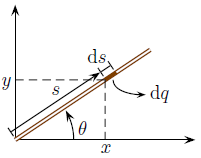
\includegraphics[width=\linewidth]{Graphics/PlanteamientoC.png}
    \vspace{-20pt}
\end{wrapfigure}

En la figura adjunta se muestra una barra de longitud
$L$, cuya carga se distribuye a lo largo de su longitud con una densidad lineal
de carga dada por $\lambda(s)=\frac{Q_{0}}{L^{2}}y$
y, donde $Q_{0}$ es una constante positiva con dimensiones
de carga y $s=s(y)$ es la longitud de arco sobre la barra expresado
en términos de la coordenada vertical $y$. Mientras que las coordenadas coordenadas
cartesianas son denotadas como $(x,y)$. Suponga que un extremo de
la barra se encuentra en el origen, además la barra está inclinada formando
un ángulo $\theta$ respecto a la horizontal; tal como se indica en la figura adjunta. También considere que la
proporción $p$ de carga distribuida en la longitud $s$ viene dada por la razón de la longitud de arco con la
longitud de la barra, es decir, $p=\frac{s}{L}$.
Sobre la base de este planteamiento responda las siguientes preguntas:

\begin{itemize}
    \item[(3a)] Seleccione todos los elementos infinitesimales de longitud de arco asociados a la longitud de la
    barra.
\end{itemize}

En base a la imagen adjunta, es posible, mediante consideraciones geom\'etricas
hallar las relaciones entre los elementos de longitud de la barra y $s$. Estos
ser\'ian: la proyecci\'on de $s$ en el eje $x$, la proyecci\'on de $s$ en el eje
$y$ y la relaci\'on $p=\frac{s}{L}$. De este modo:

\begin{equation*}
    x=s\cos\theta\Longrightarrow s=\frac{x}{\cos\theta},\qquad
    y=s\sin\theta\Longrightarrow s=\frac{y}{\sin\theta},\qquad
    p=\frac{s}{L}\Longrightarrow s=pL
\end{equation*}

Considerando que cuando varía el segmento $s$, cambian consigo los valores
de $x$, $y$ y $p$, las cantidades infinitesimales de cada relaci\'on
corresponden a:

\begin{equation*}
    \boxed{\mathrm{d}s=\frac{\mathrm{d}x}{\cos\theta}},\qquad
    \boxed{\mathrm{d}s=\frac{\mathrm{d}y}{\sin\theta}},\qquad
    \boxed{\mathrm{d}s=L\mathrm{d}p}
\end{equation*}

Por regla de la cadena, y teniendo en cuenta que:

\begin{equation*}
    \mathrm{d}s=\frac{\mathrm{d}x}{\cos\theta}
    \Longrightarrow\frac{\mathrm{d}s}{\mathrm{d}x}=\frac{1}{cos\theta}
\end{equation*}

Se tiene que:

\begin{equation*}
    \lambda(x)=\frac{\mathrm{d}Q}{\mathrm{d}x}=\frac{\mathrm{d}Q}{\mathrm{d}s}\frac{\mathrm{d}s}{\mathrm{d}x}
    =\lambda(s)\frac{\mathrm{d}s}{\mathrm{d}x}
    =\frac{Q_{0}}{L^{2}}y\frac{\mathrm{d}s}{\mathrm{d}x}
    =\frac{Q_{0}}{L^{2}}y\frac{1}{cos\theta}
    \quad\therefore\quad\boxed{\lambda(x)=\frac{Q_{0}}{L^{2}\cos\theta}y}
\end{equation*}

\begin{itemize}
    \item[(3c)] La densidad lineal de carga que la distribuye a lo largo de la longitud vertical, esto es, $\lambda(y)$.
\end{itemize}

Por regla de la cadena, y teniendo en cuenta que:

\begin{equation*}
    \mathrm{d}s=\frac{\mathrm{d}y}{\sin\theta}
    \Longrightarrow\frac{\mathrm{d}s}{\mathrm{d}y}=\frac{1}{sin\theta}
\end{equation*}

Se tiene que:

\begin{equation*}
    \lambda(y)=\frac{\mathrm{d}Q}{\mathrm{d}y}=\frac{\mathrm{d}Q}{\mathrm{d}s}\frac{\mathrm{d}s}{\mathrm{d}y}
    =\lambda(s)\frac{\mathrm{d}s}{\mathrm{d}y}
    =\frac{Q_{0}}{L^{2}}y\frac{\mathrm{d}s}{\mathrm{d}y}
    =\frac{Q_{0}}{L^{2}}y\frac{1}{sin\theta}
    \quad\therefore\quad\boxed{\lambda(y)=\frac{Q_{0}}{L^{2}\sin\theta}y}
\end{equation*}

\begin{itemize}
    \item[(3d)] Seleccione la densidad lineal de carga que la distribuye a lo largo de la longitud de la barra en
    una proporción $p$, esto es, $\lambda^{*}(p)$.
\end{itemize}

Por regla de la cadena, y teniendo en cuenta que:

\begin{equation*}
    \mathrm{d}s=L\mathrm{p}
    \Longrightarrow\frac{\mathrm{d}s}{\mathrm{d}p}=L,\qquad
    \frac{x}{\cos\theta}=\frac{y}{\sin\theta}
    \Longrightarrow y=x\frac{\sin\theta}{\cos\theta}\Longrightarrow y=x\tan\theta,\qquad
    \frac{y}{\sin\theta}=pL\Longrightarrow y=pL\sin\theta
\end{equation*}

Se tiene que:

\begin{equation*}
    \lambda(p)=\frac{\mathrm{d}Q}{\mathrm{d}p}=\frac{\mathrm{d}Q}{\mathrm{d}s}\frac{\mathrm{d}s}{\mathrm{d}p}
    =\lambda(s)\frac{\mathrm{d}s}{\mathrm{d}p}
    =\frac{Q_{0}}{L^{2}}y\frac{\mathrm{d}s}{\mathrm{d}p}
    =\frac{Q_{0}}{L^{\cancel{2}}}y\cancel{L}
    =\frac{Q_{0}}{L}y
    \quad\therefore\quad\boxed{\lambda(p)=\frac{Q_{0}}{L}y}
\end{equation*}

Por otro lado:

\begin{equation*}
    \lambda(p)=\frac{Q_{0}}{L}y
    =\frac{Q_{0}}{L}x\tan\theta
    \quad\therefore\quad\boxed{\lambda(p)=\frac{Q_{0}}{L}x\tan\theta}
\end{equation*}

Y, finalmente:

\begin{equation*}
    \lambda(p)=\frac{Q_{0}}{L}y
    =\frac{Q_{0}}{\cancel{L}}p\cancel{L}\sin\theta
    =Q_{0}p\sin\theta
    \quad\therefore\quad\boxed{\lambda(p)=Q_{0}p\sin\theta}
\end{equation*}

\begin{itemize}
    \item[(3e)] La carga contenida en todo la barra viene dada por:
\end{itemize}

Simplemente integramos cualquiera de las expresiones de $lambda$ que
conseguimos en las tres \'ultimas partes anteriores respecto a la
variable correspondiente y con los l\'imites de integraci\'on
adecuados en cada caso:

\begin{equation*}
    Q=\int_{0}^{L}\lambda(s)ds=\int_{0}^{L\cos\theta}\lambda(x)dx
    =\int_{0}^{L\sin\theta}\lambda(y)dy=\int_{0}^{1}\lambda(p)dp
\end{equation*}

Por \'ultimo:

\begin{equation*}
        Q=\int_{0}^{L}\lambda(s)\mathrm{d}s=\int_{0}^{L}\frac{Q_{0}}{L^{2}}y\mathrm{d}
        =\int_{0}^{L}\frac{Q_{0}}{L^{2}}s\sin\theta\mathrm{d}s
        =\frac{Q_{0}}{L^{2}}\sin\theta\int_{0}^{L}s\mathrm{d}s
        =\frac{Q_{0}}{\cancel{L^{2}}}\sin\theta\frac{\cancel{L^{2}}}{2}
    \quad\therefore\quad\boxed{Q=\frac{Q_{0}}{2}\sin\theta}
\end{equation*}

\section*{\underline{Planteamiento D:}}

\begin{wrapfigure}{r}{5.5cm}
    \vspace{-15pt}
    \centering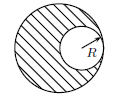
\includegraphics{Graphics/PlanteamientoD.png}
    \vspace{-20pt}
\end{wrapfigure}

En la figura adjunta se muestra un disco al cual se le hace
una perforación circular de radio $R$, considere que el diámetro del hueco coincide
con el radio del disco. El disco perforado presenta una carga positiva $Q$ distribuida
uniformemente. Sobre la base de este planteamiento responda las siguientes
preguntas:

\begin{itemize}
    \item[(5a)] La cantidad de carga necesaria para rellenar la perforación viene dada por:
\end{itemize}

Por geometr\'ia de la figura, queda claro que:

\begin{equation*}
    R=D_{h}=2R_{h}\Longrightarrow R_{h}=\frac{R}{2}
    \quad\therefore\quad A_{h}=\pi R_{h}^{2}=\pi\frac{R^{2}}{4}
\end{equation*}

Como la carga se distribuye uniformemente a lo largo de la superficie del disco,
entonces la densidad de carga superficial media del disco con el hueco corresponde
a la misma densidad de carga superficial media del hueco si suponemos que este
es un disco imaginario de mismo radio del hueco y con la misma propiedad de
carga uniformemente distribuida sobre su superficie, de esta forma:

\begin{equation*}
    \langle\lambda\rangle=\langle\lambda_{h}\rangle
    \Longrightarrow\dfrac{Q}{A-A{h}}=\dfrac{Q_{h}}{A_{h}}
    \Longrightarrow\dfrac{Q}{\pi R^{2}-\pi\frac{R^{2}}{4}}
    =\dfrac{Q_{h}}{\pi\frac{R^{2}}{4}}
    \Longrightarrow\dfrac{Q}{3\pi\frac{R^{2}}{4}}=\dfrac{Q_{h}}{\pi\frac{R^{2}}{4}}
    \quad\therefore\quad\boxed{Q_{h}=\frac{Q}{3}}
\end{equation*}

\begin{itemize}
    \item[(5a)]La cantidad de carga que tiene el disco sin perforar viene dada por:
\end{itemize}

Sumamos la carga del disco perforado con la del hueco del disco:

\begin{equation*}
    Q_{T}=Q+\frac{Q}{3}=\frac{4}{3}Q\quad\therefore\quad
    \boxed{Q_{T}=\frac{4}{3}Q}
\end{equation*}        

\section*{\underline{Planteamiento E:}}

Considere un semicírculo, de radio $R$, cuya densidad de carga superficial viene
dada por $\sigma=\sigma_{0}\frac{r^2}{R^2}$ con $r \leq R$; donde $\sigma_{0}$ es
una constante positiva con dimensiones de densidad
superficial y $r$ es la distancia radial medida desde el centro del semicírculo.

\begin{itemize}
    \item[(5a)] El elemento infinitesimal de área que se debe tomar para evitar una integral doble es:
\end{itemize}

Como $\sigma$ no depende del desplazamiento angular $\theta$ que tenga la
distancia radial r, sino solamente de este \'ultimo, entonces el
elemento infinitesimal de \'area del semic\'irculo podemos escribirlo como:

\begin{equation*}
    \mathrm{d}A=r\theta\mathrm{d}r=r\pi\mathrm{d}r
\end{equation*}

Esto, porque un semic\'irculo describe un \'angulo de $\pi$ radianes desde los
extremos radiales de su superficie.

\begin{equation*}
    \therefore\quad \boxed{\mathrm{d}A=\pi r\mathrm{d}r}
\end{equation*}

\begin{itemize}
    \item[(5b)] La densidad superficial de carga media contenida en el semicírculo viene dada por:
\end{itemize}

Primero debemos hallar la cantidad de carga distribuida por la superficie del
semic\'irculo, esto es:

\begin{equation*}
    Q=\int_{0}^{A}\sigma\mathrm{d}A=\int_{0}^{R}\sigma_{0}\frac{r^2}{R^2}\pi r\mathrm{d}r
    =\sigma_{0}\frac{\pi}{R^{2}}\int_{0}^{R}r^{3}\mathrm{d}r
    =\sigma_{0}\frac{\pi}{R^{2}}\left[\frac{R^{4}}{4}\right]
    =\sigma_{0}\frac{\pi R^{2}}{4}
\end{equation*}

Finalmente, calculamos la densidad de carga superficial media:

\begin{equation*}
    \langle\sigma\rangle=\frac{Q}{A}
    =\frac{\sigma_{0}\frac{\pi R^{2}}{4}}{\frac{\pi R^{2}}{2}}
    =\frac{\sigma_{0}\frac{\cancel{\pi R^{2}}}{4}}{\frac{\cancel{\pi R^{2}}}{2}}
    =\frac{\sigma_{0}}{2}
    \quad\therefore\quad\boxed{\langle\sigma\rangle=\frac{\sigma_{0}}{2}}
\end{equation*}

\begin{itemize}
    \item[(5b)] La carga contenida hasta una distancia radial $r \leq R$ viene dada por la expresión
\end{itemize}

Mismo procedimiento para calcular la carga en la pregunta anterior, pero esta
vez para la condici\'on $r \leq R$:

\begin{equation*}
    Q=\int_{0}^{A}\sigma\mathrm{d}A=\int_{0}^{r}\sigma_{0}\frac{r'^2}{R^2}\pi r'\mathrm{d}r'
    =\sigma_{0}\frac{\pi}{R^{2}}\int_{0}^{r}r'^{3}\mathrm{d}r'
    =\sigma_{0}\frac{\pi}{R^{2}}\left[\frac{r^{4}}{4}\right]
    =\sigma_{0}\frac{\pi r^{4}}{4R^{2}}
    \quad\therefore\quad\boxed{Q=\sigma_{0}\frac{\pi r^{4}}{4R^{2}}}
\end{equation*}

\end{document}